\chapter{Min-Cut di Karger}

\scan{54}
Il problema del \emph{taglio minimo} (\mincut) ammette un algoritmo randomizzato molto
semplice, dovuto a Karger. È un algoritmo di tipo \MonteCarlo, e lo strumento
probabilistico su cui se ne regge l'analisi è la \emph{probabilità condizionata}.

L'input è un grafo $G=(V,E)$ \emph{non orientato} e \emph{connesso}; per tutto il capitolo
poniamo $n=\abs{V}$. La richiesta di connessione non è restrittiva: su un grafo già
sconnesso il taglio minimo è vuoto e il problema è banale.

\section{Il problema}

\scan{55}

\begin{definizione}[Taglio]\label{def:taglio}
Un \emph{taglio} (\emph{cut}) $C$ di un grafo $G=(V,E)$ è un insieme di archi tale che
\begin{itemize}
  \item $C\subseteq E$;
  \item $(V,\,E\setminus C)$ è \emph{sconnesso}.
\end{itemize}
\end{definizione}

\begin{definizione}[Taglio minimo]\label{def:min-cut}
Un \emph{taglio minimo} (\emph{min-cut}) è un taglio $C$ tale che $\abs{C}$ è minima.
\end{definizione}

Si noti che si parla di taglio in senso \emph{globale} — non ci sono due terminali $s,t$
fissati — e \emph{non pesato}: il costo di un taglio è il numero dei suoi archi.

\section{Richiami: probabilità condizionata}

La probabilità condizionata è lo strumento con cui si controlla la probabilità di errore
relativa a una \emph{sequenza} di scelte, come sarà quella dell'algoritmo che stiamo per
descrivere.

\begin{itemize}
  \item Se $\mathcal{E}_1$ ed $\mathcal{E}_2$ sono \emph{indipendenti}:
  \[
    \Pr[\mathcal{E}_1\cap\mathcal{E}_2]\;=\;\Pr[\mathcal{E}_1]\cdot\Pr[\mathcal{E}_2] .
  \]
  \item Se non sono indipendenti (caso generale):
  \[
    \Pr[\mathcal{E}_1\cap\mathcal{E}_2]\;=\;\Pr[\mathcal{E}_1\mid\mathcal{E}_2]\cdot\Pr[\mathcal{E}_2],
  \]
  dove $\Pr[\mathcal{E}_1\mid\mathcal{E}_2]$ è la \emph{probabilità condizionata}: è ciò che
  ci consente di misurare la probabilità di due eventi \emph{consecutivi}.
\end{itemize}

\begin{figure}[H]
  \centering
  % prob-condizionata-venn -- due diagrammi di Venn affiancati (quaderno, pag. 55).
% A sinistra i due eventi sono disegnati disgiunti (rappresentazione informale
% dell'indipendenza, discussa nell'osservazione che segue la figura);
% a destra il caso generale, con l'intersezione non vuota evidenziata.
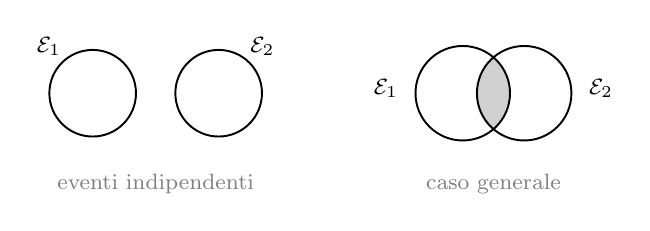
\begin{tikzpicture}[
    font=\footnotesize,
    cerchio/.style={draw,line width=0.7pt},
    didascalia/.style={font=\footnotesize,text=gray}]

  % ---- pannello sinistro: eventi che "non si influenzano" -------------------
  \begin{scope}[shift={(0,0)}]
    \draw[cerchio] (0,0)   circle[radius=0.55];
    \draw[cerchio] (1.6,0) circle[radius=0.55];
    \node[anchor=south east] at (-0.28,0.36) {$\mathcal{E}_1$};
    \node[anchor=south west] at ( 1.88,0.36) {$\mathcal{E}_2$};
    \node[didascalia] at (0.8,-1.15) {eventi indipendenti};
  \end{scope}

  % ---- pannello destro: caso generale --------------------------------------
  \begin{scope}[shift={(4.7,0)}]
    % lente d'intersezione, evidenziata
    \begin{scope}
      \clip (0,0) circle[radius=0.60];
      \fill[black!18] (0.78,0) circle[radius=0.60];
    \end{scope}
    \draw[cerchio] (0,0)    circle[radius=0.60];
    \draw[cerchio] (0.78,0) circle[radius=0.60];
    \node[anchor=east] at (-0.70,0.06) {$\mathcal{E}_1$};
    \node[anchor=west] at ( 1.48,0.06) {$\mathcal{E}_2$};
    \node[didascalia] at (0.39,-1.15) {caso generale};
  \end{scope}

\end{tikzpicture}

  \caption{A sinistra due eventi «che non si influenzano»; a destra il caso generale, con
  l'intersezione $\mathcal{E}_1\cap\mathcal{E}_2$ evidenziata.}
  \label{fig:prob-condizionata-venn}
\end{figure}

\begin{osservazione}
Nel disegno di sinistra i due eventi indipendenti sono rappresentati come regioni
\emph{disgiunte}: è solo un modo per suggerire che «non si influenzano a vicenda».
Attenzione però che l'indipendenza non ha una controparte insiemistica: due eventi disgiunti
di probabilità non nulla non sono mai indipendenti, perché
$\Pr[\mathcal{E}_1\cap\mathcal{E}_2]=0\neq\Pr[\mathcal{E}_1]\Pr[\mathcal{E}_2]$.
\end{osservazione}

Se invece di due eventi ne vogliamo misurare $m$, si itera la formula precedente e si
ottiene la \emph{regola della catena} (\emph{chain rule}):
\begin{align*}
  \Pr\!\left[\bigcap_{i=1}^{m}\mathcal{E}_i\right]
  ={}& \Pr[\mathcal{E}_1]\cdot\Pr[\mathcal{E}_2\mid\mathcal{E}_1]\cdot
       \Pr[\mathcal{E}_3\mid\mathcal{E}_1\cap\mathcal{E}_2]\cdot{}\\
     & \cdots\cdot
       \Pr\!\left[\mathcal{E}_m\;\middle|\;\bigcap_{i=1}^{m-1}\mathcal{E}_i\right].
\end{align*}
È l'unica formula probabilistica che serve per tutta l'analisi che segue: le scelte
successive dell'algoritmo non sono indipendenti, quindi la regola del prodotto non basta.

\section{L'idea: contrazione di un arco}

L'algoritmo introduce le «scelte» casuali in un modo elementare: si sceglie a caso un arco
del grafo e lo si \emph{contrae}, cioè si fondono i suoi due estremi $u$ e $v$ in un unico
nodo $uv$, che eredita tutti gli archi incidenti a $u$ o a $v$. Servono due accorgimenti:

\begin{itemize}
  \item gli archi paralleli fra due nodi distinti si mantengono tutti: si lavora perciò su
        \emph{multigrafi}, cioè su grafi in cui fra due nodi possono esserci più archi;
  \item se la contrazione forma un \emph{self-loop}, lo si ignora (viene eliminato).
\end{itemize}

\begin{figure}[H]
  \centering
  % multigrafo-archi-paralleli -- schemetto isolato (quaderno, pag. 55).
% Due nodi uniti da tre archi paralleli: la molteplicita' degli archi va
% conservata, percio' la contrazione lavora su multigrafi.
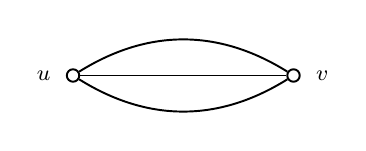
\begin{tikzpicture}[
    font=\footnotesize,
    nodo/.style={circle,draw,line width=0.7pt,fill=white,
                 inner sep=0pt,minimum size=4.5pt},
    arco/.style={line width=0.7pt}]

  \node[nodo] (u) at (0,0)   {};
  \node[nodo] (v) at (2.8,0) {};

  \draw[arco] (u) to[bend left=32]  (v);
  \draw[arco] (u) --                (v);
  \draw[arco] (u) to[bend right=32] (v);

  \node[anchor=east] at ([xshift=-2pt]u.west) {$u$};
  \node[anchor=west] at ([xshift= 2pt]v.east) {$v$};

\end{tikzpicture}

  \caption{Multigrafo: fra due nodi possono esserci più archi.}
  \label{fig:multigrafo-archi-paralleli}
\end{figure}

\begin{figure}[H]
  \centering
  % karger-contrazione -- un passo di contrazione (quaderno, pag. 55).
% Sinistra: multigrafo G con l'arco scelto (u,v) evidenziato.
% Destra:  G/(u,v): u e v fondono nel super-nodo uv; gli archi u--z e v--z
%          sopravvivono entrambi (archi paralleli), l'arco contratto diventa
%          un self-loop e viene eliminato (disegnato tratteggiato).
\begin{tikzpicture}[
    font=\footnotesize,
    nodo/.style={circle,draw,line width=0.7pt,fill=white,
                 inner sep=0pt,minimum size=4.5pt},
    arco/.style={line width=0.7pt},
    scelto/.style={line width=1.4pt},
    nota/.style={align=left,font=\footnotesize},
    glossa/.style={align=center,font=\footnotesize}]

  %% ======================= grafo di partenza G ============================
  \begin{scope}[shift={(0,0)}]
    \node[nodo] (a) at (0.0, 2.6) {};
    \node[nodo] (b) at (1.5, 3.4) {};
    \node[nodo] (v) at (3.4, 2.2) {};
    \node[nodo] (u) at (0.1, 0.6) {};
    \node[nodo] (z) at (3.2,-0.5) {};

    % archi paralleli a--b (molteplicita' 2)
    \draw[arco] (a) to[bend left=28]  (b);
    \draw[arco] (a) to[bend right=28] (b);
    % resto del multigrafo
    \draw[arco] (b) -- (v);
    \draw[arco] (a) -- (u);
    \draw[arco] (v) -- (z);
    \draw[arco] (u) -- (z);
    % arco scelto
    \draw[scelto] (u) -- (v)
      node[sloped,above=2.5pt,pos=0.44]{arco scelto};

    \node[anchor=north east] at ([shift={(-0.02,-0.04)}]u.south west) {$u$};
    \node[anchor=south west] at ([shift={( 0.04, 0.02)}]v.north east) {$v$};
    \node[anchor=north]      at ([shift={( 0.00,-0.08)}]z.south)      {$z$};
  \end{scope}

  %% =========================== freccia ondulata ===========================
  \draw[line width=0.7pt,-{Stealth[length=5pt,width=4pt]}]
        plot[domain=0:1.6,samples=90,smooth]
        ({3.78+\x},{1.20+0.075*sin(\x*900)});
  \node[glossa] at (4.58,0.62) {scelgo un arco\\e lo contraggo};

  %% ================= grafo contratto  G/(u,v) =============================
  \begin{scope}[shift={(5.9,0)}]
    \node[nodo] (aa) at (0.0, 2.6) {};
    \node[nodo] (bb) at (1.2, 3.6) {};
    \node[nodo] (uv) at (1.6, 1.3) {};
    \node[nodo] (zz) at (2.9,-0.4) {};

    % la lente a--b sopravvive invariata
    \draw[arco] (aa) to[bend left=28]  (bb);
    \draw[arco] (aa) to[bend right=28] (bb);
    % eredi di b--v e di a--u
    \draw[arco] (bb) -- (uv);
    \draw[arco] (aa) -- (uv);
    % eredi di v--z e u--z: due archi paralleli
    \draw[arco] (uv) to[bend left=32]  (zz);
    \draw[arco] (uv) to[bend right=32] (zz);
    % self-loop generato dalla contrazione: eliminato
    \draw[arco,dash pattern=on 1.6pt off 1.6pt]
          (uv) .. controls +(0.95,0.75) and +(0.95,-0.75) .. (uv);

    \node[anchor=east] at ([shift={(-0.22,0.06)}]uv.west) {$uv$};
    \node[anchor=north west] at ([shift={( 0.04,-0.04)}]zz.south east) {$z$};

    \draw[line width=0.5pt] (2.30,1.56) -- (2.82,1.92);
    \node[nota,anchor=west] at (2.88,2.00)
         {se formo un\\self-loop,\\lo ignoro};
  \end{scope}

\end{tikzpicture}

  \caption{Un passo dell'algoritmo: si sceglie a caso l'arco $(u,v)$ e lo si contrae. Gli
  archi $u$--$z$ e $v$--$z$ diventano due archi paralleli fra $uv$ e $z$; l'arco contratto
  diventa un self-loop e viene eliminato.}
  \label{fig:karger-contrazione}
\end{figure}

Mantenere gli archi paralleli è essenziale: la molteplicità del fascio che unisce due
super-nodi conta esattamente quanti archi \emph{originali} di $G$ hanno un estremo in
ciascuno dei due insiemi di vertici che quei super-nodi rappresentano.

\scan{56}
Ripetendo l'operazione, dopo $n-2$ contrazioni si arriva a questa situazione:

\begin{figure}[H]
  \centering
  % karger-due-nodi-taglio -- situazione dopo n-2 contrazioni (quaderno, pag. 56).
% Restano due super-nodi a e b uniti da quattro archi paralleli; la linea
% ondulata verticale li attraversa tutti: quel fascio di archi e' un taglio
% del grafo di partenza.
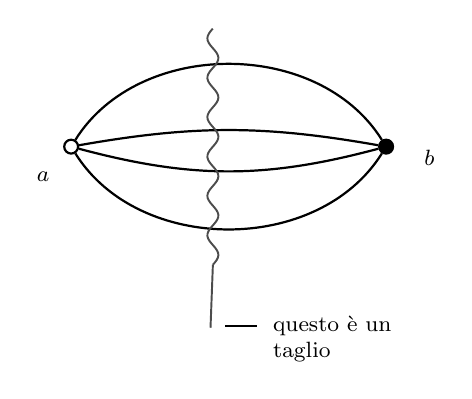
\begin{tikzpicture}[
    font=\footnotesize,
    nodo/.style={circle,draw,line width=0.8pt,fill=white,
                 inner sep=0pt,minimum size=5pt},
    nodopieno/.style={circle,draw,line width=0.8pt,fill=black,
                 inner sep=0pt,minimum size=5pt},
    arco/.style={line width=0.8pt},
    taglio/.style={line width=0.7pt,black!70}]

  % ---- i due super-nodi residui --------------------------------------------
  \node[nodo]      (a) at (0,0) {};
  \node[nodopieno] (b) at (4,0) {};
  \node[anchor=north east] at ([shift={(-0.08,-0.12)}]a.south west) {$a$};
  \node[anchor=west]       at ([shift={( 0.26,-0.14)}]b.east)       {$b$};

  % ---- fascio di quattro archi paralleli -----------------------------------
  \draw[arco] (a) to[bend left=58]  (b);
  \draw[arco] (a) to[bend left=10]  (b);
  \draw[arco] (a) to[bend right=15] (b);
  \draw[arco] (a) to[bend right=58] (b);

  % ---- linea di taglio: serpentina verticale, tracciata sopra gli archi ----
  \draw[taglio] plot[domain=-1.50:1.50,samples=100,smooth]
        ({1.80+0.07*sin(\x*720)},{\x});
  \draw[taglio] (1.80,-1.50) -- (1.77,-2.30);

  % ---- annotazione ---------------------------------------------------------
  \draw[line width=0.5pt] (1.96,-2.28) -- (2.36,-2.28);
  \node[anchor=west,align=left] at (2.44,-2.44) {questo è un\\taglio};

\end{tikzpicture}

  \caption{Dopo $n-2$ contrazioni restano due soli nodi, $a$ e $b$, uniti da un fascio di
  archi paralleli: \emph{questo è un taglio} del grafo di partenza.}
  \label{fig:karger-due-nodi-taglio}
\end{figure}

\begin{algorithm}[H]
\caption{\contract: una singola esecuzione dell'algoritmo randomizzato di Karger per il \mincut}
\label{alg:contract}
\begin{algorithmic}[1]
  \Require un multigrafo non orientato e connesso $G=(V,E)$, con $n=\abs{V}$
  \Ensure un insieme di archi che è un taglio di $G$
  \For{$i \gets 1$ \textbf{to} $n-2$}
    \State scegli uniformemente a caso un arco $(u,v)\in E$
    \State cancella $u$ e $v$ da $V$ e introduci un nuovo nodo $uv$
      \Comment{contrazione: $\Oh(1)$}
    \State reindirizza su $uv$ ogni arco incidente su $u$ o su $v$
    \State elimina i self-loop che si sono generati
  \EndFor
  \State \Return gli archi fra i $2$ nodi rimasti
\end{algorithmic}
\end{algorithm}

\begin{osservazione}
L'annotazione $\Oh(1)$ per il costo di una contrazione va presa con cautela: se il
multigrafo è rappresentato esplicitamente, reindirizzare tutti gli archi incidenti su $u$ e
su $v$ costa $\Oh(n)$ e una singola esecuzione dell'algoritmo costa $\Oh(n^{2})$. Il costo
costante va riferito alla sola fusione dei due nodi, e lo si ottiene con una realizzazione
«pigra»: si tiene la lista degli archi di partenza, si fondono i nodi con una
\emph{union--find} e si scartano gli archi diventati self-loop soltanto nel momento in cui
vengono estratti. Anche così, però, il guadagno riguarda solo i grafi sparsi: il costo
complessivo di una singola esecuzione resta $\Om(\abs{E})$, e sui grafi densi
$\abs{E}=\Th(n^{2})$, quindi non si guadagna nulla rispetto alla rappresentazione
esplicita.
\end{osservazione}

L'algoritmo è \emph{corretto per costruzione}: qualunque siano le scelte casuali, ciò che
restituisce è sempre un taglio di $G$. L'unica cosa aleatoria è se sia \emph{minimo}.

\begin{lemma}[gli archi residui formano un taglio]\label{lem:taglio-residuo}
L'insieme $F$ degli archi fra i due nodi rimasti dopo $n-2$ contrazioni è un taglio di $G$.
\end{lemma}

\begin{dimostrazione*}
Siano $a$ e $b$ i due nodi rimasti dopo le $n-2$ contrazioni, e siano
$\{a_1,\dots,a_p\}$ e $\{b_1,\dots,b_q\}$ i nodi di $G$ contratti rispettivamente su $a$ e
su $b$. I due insiemi sono non vuoti e costituiscono una bipartizione di $V$.

Una contrazione non cancella mai un arco i cui estremi finiscono in parti diverse: le
uniche cancellazioni sono quelle dei self-loop, cioè degli archi i cui due estremi sono già
stati fusi nello stesso super-nodo. Ogni arco di $G$ con un estremo in $\{a_1,\dots,a_p\}$
e l'altro in $\{b_1,\dots,b_q\}$ sopravvive dunque fino alla fine, e gli archi paralleli
fra $a$ e $b$ — cioè $F$ — sono esattamente questi.

Ne segue che ogni cammino in $G$ da un $a_i$ a un $b_j$ deve attraversare un arco di $F$:
rimosso $F$, nessun $a_i$ è più collegato ad alcun $b_j$, quindi $(V,E\setminus F)$ è
sconnesso e $F$ è un taglio di $G$.
\end{dimostrazione*}

\begin{figure}[H]
  \centering
  % karger-bipartizione-taglio -- pag. 56
% La bipartizione di V indotta dalle n-2 contrazioni: a sinistra i nodi fusi nel
% super-nodo a, a destra quelli fusi in b. La linea ondulata e' il taglio F
% restituito dall'algoritmo: ogni cammino da un a_i a un b_j e' costretto ad
% attraversarla.  (Nel quaderno questo insieme e' chiamato C; nel capitolo C e'
% riservato al taglio minimo fissato per l'analisi.)
% NB: nel quaderno i pedici sono k e h; qui sono p e q, per non collidere con
% k = |C| e con l'h del numero di ripetizioni.
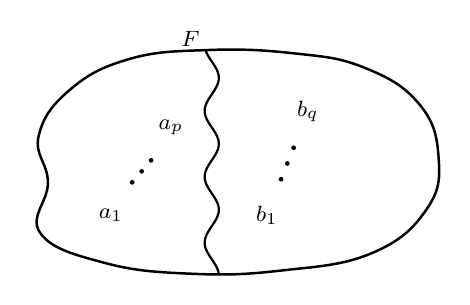
\begin{tikzpicture}[x=1cm,y=1cm,line join=round,line cap=round,font=\footnotesize]

  % sagoma dell'insieme V (contorno irregolare, "a mano libera")
  \def\sagoma{plot[smooth cycle,tension=0.72] coordinates {
      (2.60,0.05) (2.35,0.72) (1.65,1.18) (0.75,1.36) (-0.35,1.40) (-1.35,1.28)
      (-2.10,0.88) (-2.48,0.30) (-2.36,-0.28) (-2.46,-0.92) (-1.65,-1.30)
      (-0.55,-1.44) (0.60,-1.40) (1.75,-1.18) (2.45,-0.62)}}

  \draw[line width=0.9pt] \sagoma;

  % ---- il taglio F: frontiera ondulata fra le due classi -------------------
  % la serpentina si disegna piu' lunga della sagoma e si taglia sul bordo
  \begin{scope}
    \clip \sagoma;
    \draw[line width=0.8pt] plot[domain=-1.70:1.70,samples=140,smooth]
          ({-0.28+0.09*sin(\x*430)},{\x});
  \end{scope}
  \node[anchor=south,inner sep=1.5pt] at (-0.55,1.38) {$F$};

  % ---- classe dei nodi contratti su a (a sinistra del taglio) --------------
  \node[inner sep=1pt] at (-1.56,-0.70) {$a_{1}$};
  \fill (-1.29,-0.28) circle (0.85pt);
  \fill (-1.17,-0.14) circle (0.85pt);
  \fill (-1.05, 0.00) circle (0.85pt);
  \node[inner sep=1pt] at (-0.80, 0.42) {$a_{p}$};

  % ---- classe dei nodi contratti su b (a destra del taglio) ---------------
  \node[inner sep=1pt] at ( 0.42,-0.70) {$b_{1}$};
  \fill ( 0.60,-0.24) circle (0.85pt);
  \fill ( 0.68,-0.04) circle (0.85pt);
  \fill ( 0.76, 0.16) circle (0.85pt);
  \node[inner sep=1pt] at ( 0.94, 0.62) {$b_{q}$};

\end{tikzpicture}

  \caption{La bipartizione di $V$ indotta dalle contrazioni: a sinistra i nodi contratti su
  $a$, a destra quelli contratti su $b$. La linea ondulata è il taglio $F$, e ogni cammino
  da un $a_i$ a un $b_j$ è costretto ad attraversarla.}
  \label{fig:karger-bipartizione-taglio}
\end{figure}

\section{Analisi: quando il taglio restituito è minimo}

\scan{57}

\begin{domanda}
Qual è la probabilità che il taglio $F$ restituito dall'algoritmo sia un \emph{taglio
minimo}, e non semplicemente un taglio qualunque?
\end{domanda}

\begin{figure}[H]
  \centering
  % mincut-schema-taglio -- pag. 57
% Il grafo G con un suo taglio C (la serpentina verticale). A sinistra una zona
% rada, a destra un cluster denso (un K_4); soltanto due archi attraversano la
% frontiera, quindi |C| = 2. E' questo squilibrio fra archi interni e archi del
% taglio a rendere probabile che una contrazione casuale non distrugga C.
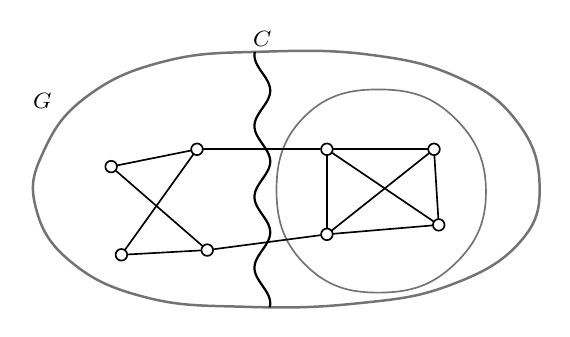
\begin{tikzpicture}[x=1cm,y=1cm,line join=round,line cap=round,
    font=\footnotesize,
    nodo/.style={circle,draw,line width=0.6pt,fill=white,
                 inner sep=0pt,minimum size=4.2pt},
    arco/.style={line width=0.6pt},
    contorno/.style={line width=0.9pt,black!55}]

  % sagoma del grafo G
  \def\sagoma{plot[smooth cycle,tension=0.72] coordinates {
      (3.20,-0.05) (2.90,0.75) (2.15,1.30) (1.05,1.58) (-0.30,1.62) (-1.55,1.50)
      (-2.55,1.05) (-3.10,0.35) (-3.20,-0.35) (-2.75,-1.05) (-1.80,-1.50)
      (-0.55,-1.62) (0.85,-1.58) (2.05,-1.35) (2.95,-0.80)}}

  \draw[contorno] \sagoma;
  \node[anchor=east,inner sep=2pt] at (-2.92,1.00) {$G$};

  % ---- il taglio: serpentina verticale, tagliata sul bordo della sagoma ----
  \begin{scope}
    \clip \sagoma;
    \draw[line width=0.8pt] plot[domain=-1.90:1.90,samples=150,smooth]
          ({-0.32+0.10*sin(\x*400)},{\x});
  \end{scope}
  \node[anchor=south,inner sep=1.5pt] at (-0.32,1.62) {$C$};

  % ---- parte sinistra: rada ------------------------------------------------
  \node[nodo] (A) at (-2.24, 0.16) {};
  \node[nodo] (B) at (-1.15, 0.38) {};
  \node[nodo] (D) at (-2.11,-0.96) {};
  \node[nodo] (F) at (-1.02,-0.90) {};

  \draw[arco] (A) -- (B);
  \draw[arco] (A) -- (F);   % le due diagonali
  \draw[arco] (B) -- (D);   % si incrociano
  \draw[arco] (D) -- (F);

  % ---- parte destra: cluster denso (K_4) -----------------------------------
  \draw[contorno,line width=0.6pt]
        plot[smooth cycle,tension=0.75] coordinates {
          (2.52,-0.16) (2.12,0.78) (1.18,1.14) (0.22,0.80) (-0.14,-0.16)
          (0.24,-1.10) (1.18,-1.44) (2.12,-1.08)};

  \node[nodo] (P) at (0.50, 0.38) {};
  \node[nodo] (Q) at (1.86, 0.38) {};
  \node[nodo] (R) at (1.92,-0.58) {};
  \node[nodo] (S) at (0.50,-0.70) {};

  \draw[arco] (P) -- (Q);
  \draw[arco] (Q) -- (R);
  \draw[arco] (R) -- (S);
  \draw[arco] (S) -- (P);
  \draw[arco] (P) -- (R);
  \draw[arco] (Q) -- (S);

  % ---- gli unici due archi che attraversano il taglio ----------------------
  \draw[arco] (B) -- (P);
  \draw[arco] (F) -- (S);

\end{tikzpicture}

  \caption{Il grafo $G$ e un suo taglio (la linea ondulata): la grande maggioranza degli
  archi è \emph{interna} alle due parti, pochissimi attraversano il taglio. È questo
  squilibrio a rendere probabile che una contrazione scelta a caso \emph{non} distrugga il
  taglio.}
  \label{fig:mincut-schema-taglio}
\end{figure}

\begin{dubbio}
Accanto al disegno, a matita e ormai quasi cancellata, c'è un'annotazione di quattro righe
collegata alla figura da una linea di richiamo. Se ne leggono con ragionevole sicurezza solo
l'inizio, «alta prob.\ che contra\dots», e l'ultima riga, «\dots\ da solo»; il resto non è
ricostruibile. Il senso, coerente con il disegno e con il resto della pagina, è che con alta
probabilità la contrazione cade su un arco \emph{interno} a una delle due parti e non su un
arco del taglio.
\end{dubbio}

\subsection{Gli eventi \texorpdfstring{$\mathcal{E}_i$}{E\_i} e il primo passo}

\begin{definizione}[Scelta positiva o negativa; evento $\mathcal{E}_i$]\label{def:evento-Ei}
Sia $\mathcal{E}_i$ l'evento «la scelta dell'$i$-esimo arco da contrarre è \emph{positiva}»,
dove una scelta si dice
\begin{itemize}
  \item \emph{positiva} se dopo la contrazione rimango dentro un taglio minimo, cioè se
        l'arco estratto \emph{non} appartiene al taglio minimo che voglio preservare;
  \item \emph{negativa} altrimenti.
\end{itemize}
\end{definizione}

Quello che serve calcolare è dunque la probabilità di rimanere dentro un taglio minimo al
passo $i$, cioè la probabilità dell'evento $\mathcal{E}_i$: e, come si vedrà, questa va
condizionata all'esito positivo di tutte le scelte precedenti, perché le contrazioni
successive non sono fra loro indipendenti.

\begin{figure}[H]
  \centering
  % mincut-c-in-e -- pag. 57
% Il taglio minimo C come sottoinsieme dell'insieme E degli archi: l'arco da
% contrarre e' estratto uniformemente a caso da E, quindi la probabilita' di
% colpire un arco di C e' |C|/|E|, e il disegno rende visivo che tale rapporto
% e' piccolo.
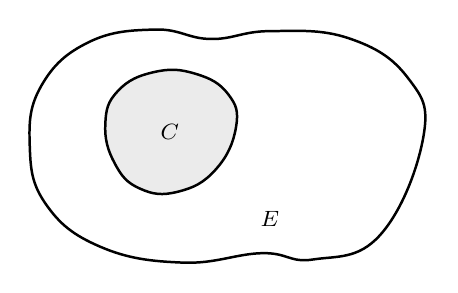
\begin{tikzpicture}[x=1cm,y=1cm,line join=round,line cap=round,font=\footnotesize]

  % ---- l'insieme E degli archi --------------------------------------------
  \draw[line width=0.9pt] plot[smooth cycle,tension=0.72] coordinates {
      (2.50,0.10) (2.30,0.85) (1.55,1.35) (0.55,1.44) (-0.20,1.34) (-0.90,1.46)
      (-1.75,1.30) (-2.35,0.75) (-2.50,0.00) (-2.30,-0.75) (-1.60,-1.30)
      (-0.55,-1.50) (0.45,-1.38) (1.10,-1.46) (1.95,-1.15)};
  \node[inner sep=1pt] at (0.55,-0.95) {$E$};

  % ---- il taglio minimo C --------------------------------------------------
  \draw[line width=0.9pt,fill=black!8] plot[smooth cycle,tension=0.75] coordinates {
      (0.12,0.22) (0.02,0.64) (-0.40,0.90) (-0.92,0.92) (-1.38,0.68)
      (-1.54,0.26) (-1.42,-0.24) (-1.10,-0.56) (-0.62,-0.60) (-0.14,-0.32)};
  \node[inner sep=1pt] at (-0.72,0.16) {$C$};

\end{tikzpicture}

  \caption{Il taglio minimo $C$ come sottoinsieme di $E$: l'arco da contrarre viene estratto
  uniformemente a caso da $E$, quindi la probabilità di colpire proprio un arco di $C$ è
  $\abs{C}/\abs{E}$.}
  \label{fig:mincut-c-in-e}
\end{figure}

Nel caso peggiore il grafo ha un \emph{unico} taglio minimo $C$: la probabilità di scegliere
proprio un arco di quel taglio è
\[
  \frac{\abs{C}}{\abs{E}} ,
\]
e di $C$ interessa soltanto la cardinalità. Se i tagli minimi fossero più d'uno, per
sbagliare occorrerebbe distruggerli tutti e la probabilità di errore sarebbe minore: il caso
di un unico taglio minimo è quindi davvero il peggiore. Fissiamo allora un taglio minimo $C$
e poniamo $k=\abs{C}$; ricordiamo che $n=\abs{V}$.

\begin{osservazione}
Per ogni vertice $v$ vale $d(v) \ge k$.

Altrimenti l'insieme degli archi incidenti a $v$ — che è già un taglio, quello che «taglia
fuori» il solo nodo $v$ — avrebbe cardinalità $d(v) < k$: assurdo, perché $k$ è la
cardinalità minima di un taglio di $G$.
\end{osservazione}

Sommando i gradi di tutti i vertici ogni arco viene contato due volte, quindi
$2\abs{E} = \sum_{v \in V} d(v) \ge n\,k$, da cui
\[
  \abs{E} \;\ge\; \frac{k \cdot n}{2}
  \qquad\Longrightarrow\qquad
  \frac{\abs{C}}{\abs{E}} \;\le\; \frac{k}{\dfrac{k \cdot n}{2}} \;=\; \frac{2}{n} .
\]

Il valore $2/n$ è dunque un maggiorante della probabilità dell'evento complementare
$\overline{\mathcal{E}_1}$, cioè della probabilità di distruggere il taglio minimo già alla
prima contrazione:
\[
  \Pr\bigl[\,\overline{\mathcal{E}_1}\,\bigr] \;\le\; \frac{2}{n} .
\]

\scan{58}
Ne segue che la probabilità che, dopo la prima contrazione, esista ancora un taglio minimo
che l'algoritmo può determinare è
\[
  \Pr[\mathcal{E}_1] \;\ge\; 1-\frac{2}{n} .
\]

\subsection{I passi successivi}

Indichiamo con $G_i$ il multigrafo ottenuto dopo $i$ contrazioni ($G_0=G$) e con $E_i$ il suo
insieme di archi.

Passiamo alla seconda contrazione. Il multigrafo $G_1$ ha $n-1$ nodi e, condizionatamente a
$\mathcal{E}_1$, ammette ancora $C$ come taglio minimo, di cardinalità $k$. Ogni nodo di
$G_1$ ha quindi grado almeno $k$, per cui
\[
  \abs{E_1}\;\ge\;\frac{k\,(n-1)}{2}
  \qquad\Longrightarrow\qquad
  \Pr\!\left[\overline{\mathcal{E}_2}\;\middle|\;\mathcal{E}_1\right]
  \;\le\;\frac{\abs{C}}{\abs{E_1}}
  \;\le\;\frac{k}{\dfrac{k\,(n-1)}{2}}
  \;=\;\frac{2}{n-1},
\]
e passando all'evento complementare
\[
  \Pr[\mathcal{E}_2\mid\mathcal{E}_1]\;\ge\;1-\frac{2}{n-1}.
\]

\begin{osservazione}
Il passaggio si ripete identico a ogni passo perché una contrazione non può \emph{diminuire}
il valore del taglio minimo: ogni taglio del multigrafo contratto $G_i$ è anche un taglio di
$G$, e quindi contiene almeno $k$ archi. Finché non si contrae un arco di $C$, il taglio
minimo di $G_i$ vale esattamente $k$, ogni nodo di $G_i$ ha grado $\ge k$ e vale di nuovo la
stima sul numero di archi.
\end{osservazione}

In generale, dopo $i-1$ contrazioni restano $n-(i-1)=n-i+1$ nodi, dunque
$\abs{E_{i-1}}\ge k\,(n-i+1)/2$ e
\[
  \Pr\!\left[\mathcal{E}_i \;\middle|\; \bigcap_{j=1}^{i-1}\mathcal{E}_j\right]
  \;\ge\; 1-\frac{2}{n-i+1}.
\]

\subsection{Probabilità di successo di una singola esecuzione}

\begin{teorema}[Karger]\label{thm:karger}
Fissato un taglio minimo $C$ di $G$, una singola esecuzione di \contract restituisce
proprio $C$ con probabilità
\[
  \Pr\!\left[\bigcap_{i=1}^{n-2}\mathcal{E}_i\right]
  \;\ge\; \frac{2}{n(n-1)} \;=\; \frac{1}{\binom{n}{2}} \;\ge\; \frac{2}{n^{2}} .
\]
\end{teorema}

\begin{dimostrazione*}
La quantità che interessa è la probabilità che la scelta dell'arco da contrarre sia
\emph{positiva} a \emph{ogni} passo, cioè $\Pr\bigl[\bigcap_{i=1}^{n-2}\mathcal{E}_i\bigr]$:
poiché le scelte successive non sono indipendenti, la si calcola con la regola della catena.
\begin{align*}
  \Pr\!\left[\bigcap_{i=1}^{n-2}\mathcal{E}_i\right]
  &= \Pr[\mathcal{E}_1]\cdot\Pr[\mathcal{E}_2\mid\mathcal{E}_1]\cdot\;\cdots\;\cdot
     \Pr\!\left[\mathcal{E}_{n-2}\;\middle|\;\bigcap_{i=1}^{n-3}\mathcal{E}_i\right]\\[4pt]
  &\ge \left(1-\frac{2}{n}\right)\left(1-\frac{2}{n-1}\right)\cdot\;\cdots\;\cdot
       \left(1-\frac{2}{\,n-(n-2)+1\,}\right)\\[4pt]
  &= \left(\frac{n-2}{n}\right)\left(\frac{n-3}{n-1}\right)\left(\frac{n-4}{n-2}\right)
     \cdots\;\frac{2}{4}\cdot\frac{1}{3}
   \;=\;\frac{2}{n(n-1)} ,
\end{align*}
dove l'ultimo passaggio segue dal fatto che il prodotto è telescopico: ogni numeratore si
semplifica con il denominatore che compare due fattori più avanti, e sopravvivono soltanto i
numeratori $2$ e $1$ degli ultimi due fattori e i denominatori $n$ e $n-1$ dei primi due.
Infine $n(n-1)\le n^{2}$ dà l'ultima disuguaglianza.
\end{dimostrazione*}

La probabilità di successo è dunque solo \emph{inversamente polinomiale} in $n$, non
esponenzialmente piccola: è precisamente questo a rendere efficace l'amplificazione per
ripetizione.

\section{Amplificazione per ripetizione}

\begin{osservazione}
La probabilità che il taglio restituito da \contract \emph{non} sia minimo è
\[
  \begin{aligned}
    \text{dopo un'esecuzione:}   &\quad \le\; 1-\frac{2}{n^{2}},\\[4pt]
    \text{dopo due esecuzioni:}  &\quad \le\; \left(1-\frac{2}{n^{2}}\right)^{\!2},\\[4pt]
    \text{dopo $h$ esecuzioni:}  &\quad \le\; \left(1-\frac{2}{n^{2}}\right)^{\!h}.
  \end{aligned}
\]
Le $h$ esecuzioni sono infatti indipendenti fra loro — a differenza dei passi \emph{interni}
a una singola esecuzione — e si restituisce il migliore degli $h$ tagli trovati: si sbaglia
soltanto se sbagliano tutte, da cui il prodotto delle probabilità di errore.
\end{osservazione}

\begin{figure}[H]
  \centering
  % karger-tradeoff -- pag. 58
% Il compromesso dell'amplificazione per ripetizione: al crescere del numero h
% di esecuzioni indipendenti sale il costo (freccia verso l'alto) e scende la
% probabilita' di errore (freccia verso il basso).
% Nel quaderno le etichette sono abbreviate («maggior complessità», «minore
% prob. di errore»): qui sono espanse.
\begin{tikzpicture}[x=1cm,y=1cm,line cap=round,font=\footnotesize,
    >={Stealth[length=5pt,width=4pt]}]

  % ---- costo: cresce -------------------------------------------------------
  \draw[->,line width=0.8pt] (0,0) -- (0,1.55);
  \node[anchor=west,inner sep=5pt] at (0.10,1.45) {maggiore complessità computazionale};

  % ---- probabilità di errore: cala ----------------------------------------
  \draw[->,line width=0.8pt] (0,-0.75) -- (0,-2.30);
  \node[anchor=west,inner sep=5pt] at (0.10,-2.20) {minore probabilità di errore};

\end{tikzpicture}

  \caption{Il compromesso fra costo e affidabilità: al crescere del numero $h$ di ripetizioni
  aumenta la complessità computazionale e diminuisce la probabilità di errore.}
  \label{fig:karger-tradeoff}
\end{figure}

\scan{59}
Resta da fissare il numero $h$ di ripetizioni indipendenti. Prendendo
\[
  h \;=\; \frac{n^{2}}{2}
\]
si ottiene
\[
  \left(1-\frac{1}{\,n^{2}/2\,}\right)^{\!n^{2}/2}
  \;=\;\left(1-\frac{2}{n^{2}}\right)^{\!n^{2}/2}
  \;<\;\frac{1}{e},
\]
cioè la probabilità che \emph{nessuna} delle $h$ esecuzioni abbia prodotto un taglio minimo
scende sotto $1/e$.

\begin{osservazione}
La disuguaglianza è il caso $m=n^{2}/2$ della stima
$\bigl(1-\tfrac{1}{m}\bigr)^{m}<e^{-1}$, valida per ogni $m>1$ e conseguenza immediata di
$1-x<e^{-x}$ — vera per ogni $x\neq 0$ — posto $x=\tfrac{1}{m}$.
\end{osservazione}

Numericamente
\[
  \frac{1}{e}\;\approx\;\frac{1}{3}\;\approx\;0{,}33
\]
(più precisamente $1/e\approx 0{,}368$): con $h=n^{2}/2$ ripetizioni la probabilità di errore
è dunque una \emph{costante} minore di $1$, indipendente da $n$. Trattandosi di una costante,
la si abbatte quanto si vuole continuando a iterare: con
$h=\frac{n^{2}}{2}\ln\frac{1}{\delta}$ esecuzioni la probabilità di errore è al più $\delta$.

\begin{osservazione}
Mettendo insieme le due stime si legge in cifre il compromesso della
\autoref{fig:karger-tradeoff}: una singola esecuzione di \contract costa $\Oh(n^{2})$ con la
rappresentazione esplicita del multigrafo, quindi $h=n^{2}/2$ ripetizioni costano
$\Oh(n^{4})$ per una probabilità di errore inferiore a $1/e$, e
$h=\Th(n^{2}\log n)$ ripetizioni costano $\Oh(n^{4}\log n)$ per una probabilità di errore
polinomialmente piccola.
\end{osservazione}
